\documentclass[12pt]{article}
\usepackage{graphicx}
%\documentclass[journal,12pt,twocolumn]{IEEEtran}
\usepackage[none]{hyphenat}
\usepackage{graphicx}
\usepackage{listings}
\usepackage[english]{babel}
\usepackage{graphicx}
\usepackage{caption}
\usepackage[parfill]{parskip}
\usepackage{hyperref}
\usepackage{booktabs}
\usepackage{gensymb}
%\usepackage{setspace}\doublespacing\pagestyle{plain}
\def\inputGnumericTable{}
\usepackage{color}                                            %%
    \usepackage{array}                                            %%
    \usepackage{longtable}                                        %%
    \usepackage{calc}                                             %%
    \usepackage{multirow}                                         %%
    \usepackage{hhline}                                           %%
    \usepackage{ifthen}
\usepackage{array}
\usepackage{amsmath}   % for having text in math mode
\usepackage{parallel,enumitem}
\usepackage{listings}
\lstset{
language=tex,
frame=single,
breaklines=true
}
 
%Following 2 lines were added to remove the blank page at the beginning
\usepackage{atbegshi}% http://ctan.org/pkg/atbegshi
\AtBeginDocument{\AtBeginShipoutNext{\AtBeginShipoutDiscard}}
%
%New macro definitions
\newcommand{\mydet}[1]{\ensuremath{\begin{vmatrix}#1\end{vmatrix}}}
\providecommand{\brak}[1]{\ensuremath{\left(#1\right)}}
\providecommand{\norm}[1]{\left\lVert#1\right\rVert}
\newcommand{\solution}{\noindent \textbf{Solution: }}
\newcommand{\myvec}[1]{\ensuremath{\begin{pmatrix}#1\end{pmatrix}}}
\let\vec\mathbf
\begin{document}
\begin{center}
\enlargethispage{-4cm}
\title{\textbf{Vector Algebra}}
\date{\vspace{-5ex}} %Not to print date automatically
\maketitle
\end{center}
\setcounter{page}{1}
\section*{12$^{th}$ Maths - Chapter 10}
This is Problem-3 from Exercise 10.4
\begin{enumerate}
\item A girl walks $4$ km towards west, then she walk $3$ km in a direction $30\degree$ east of north and stops. Determine the girl's displacement from her initial point of departure.

\solution 
		Let initial point, middile point, final point be $\vec{A}, \vec{B}$ and $\vec{C}$ respectively. Let initial point be the origin,  
\begin{align}
	\vec{A}=\myvec{0\\0}
	\end{align}
Now, girl walks $4$km towards west $\vec{A}$-$\vec{B}$ then,
		\begin{align}
			\Vec{A}\text{-}\Vec{B}=\myvec{-4\\0}
\end{align}
Then girl walks 3 km in the direction $30\degree$ east of north
 \begin{align}
	 \Vec{B}\text{-}\vec{C}&=\myvec{3\cos{60\degree}\\3\sin{60\degree}}\\
&=\myvec{\frac{3}{2}\\ \frac{3\sqrt{3}}{2}}
 \end{align}
 By triangle law of vector addition, we have
\begin{align}
	\vec{A}\text{-}\Vec{C} &= \vec{A}\text{-}\Vec{B}+\vec{B}\text{-}\Vec{C}\\
 &=\myvec{-4\\0}+\myvec{\frac{3}{2}\\[2pt] \frac{3\sqrt{3}}{2}}\\
 &=\myvec{\frac{-5}{2}\\[2pt] \frac{3\sqrt{3}}{2}}
\end{align}
  Hence, the girl's displacement from her initial point of departure is 
\begin{align}
\myvec{\frac{-5}{2}\\[2pt] \frac{3\sqrt{3}}{2}}
\end{align}

\begin{figure}[!h] 
 \begin{center} 
 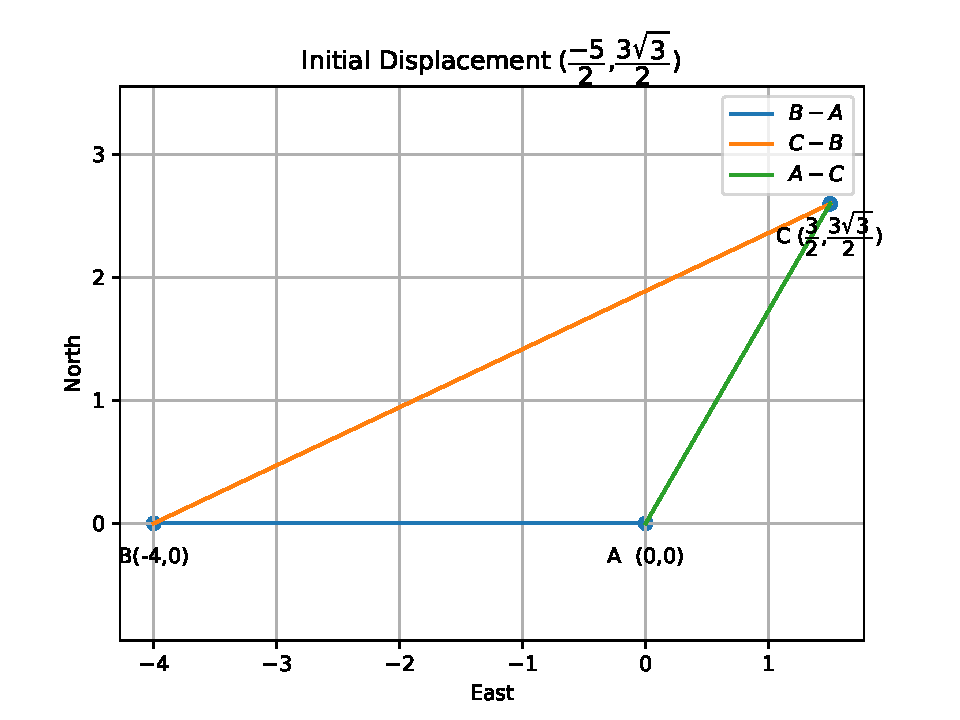
\includegraphics[width=\columnwidth]{figs/fig.pdf} 
 \end{center} 
\caption{} 
\label{fig:Fig1} 
\end{figure}
\end{enumerate}
\end{document}
